\documentclass[a4paper,14pt]{report}
\usepackage[spanish]{babel}
\selectlanguage{spanish}
\usepackage[utf8]{inputenc} 
\usepackage[dvips]{graphicx}
\graphicspath{{images/}}
\usepackage{float} % para usar [H]
\usepackage{hyperref}
%%%%%%%%%%%%%%%%%%%%%%%%%%%%%%%%%%%%%%%%%%%%%%%%%%%%%%%%%%%%%%%%%%%%%%%%%%%%%%%
% Chapter 2: Descripción de la aplicación: ChefManagement
%%%%%%%%%%%%%%%%%%%%%%%%%%%%%%%%%%%%%%%%%%%%%%%%%%%%%%%%%%%%%%%%%%%%%%%%%%%%%%%
\begin{document}
\chapter{Descripción de la aplicaci\'on}\label{dos}

En el capítulo anterior~\ref{chapter:intro} se ha introducido tanto los antecedentes como se describió brevemente la aplicación. En este capítulo explicaremos toda las funcionalidades y sus características con detalle. \\

Partimos de qué tipo de aplicación queremos crear. Se trata de desarrollar un software que ayude a las personas a gestionar el costo de producción de las recetas, dependiendo del precio de sus ingredientes y el número de raciones. Ésta se llamará \textbf{ChefManagement} y sus características iniciales son:
\begin{itemize}
	\item Crear, ver, editar y eliminar recetas.
	\item Listar todas las recetas.
	\item Crear backup de las recetas y cargarlo si es necesario.
	\item Calcular el precio de una determinada receta para un determinado número de comensales.
\end{itemize}

Para esta primera versión, además de ser capaz de realizar esta serie de tareas, debe  cumplir con las necesidades y espectativas del usuario y facilitar su interacción con la aplicación. Éstos son sus requisitos iniciales:
\begin{itemize}
	\item Dos entornos de producción: la aplicación puede ser usada desde dos nubes diferentes.
	\item Tener en cuenta aspectos de usablidad: adaptación, entendimiento y facilidad de uso.
	\item Importar y exportar archivos en formato json: almacenar copias de las recetas en el equipo cliente y restaurarlas si es necesario.
	\item Accesso mediante registro o haciendo uso de APIs de distintas redes sociales como Google+ o Facebook. Hay que facilitar el acceso a los usuarios.
\end{itemize}

Tanto las características comos los requisitos de la aplicación serán aplicadas a la versión 1.0, pudiendo ser mejorados o añadidos más en futuras versiones~\ref{chapter:cinco}.

\vspace*{0.2in}
\section{Acceso a la aplicación}\label{cap.2.1}

Para usar esta aplicación podemos acceder directamente a sus entornos de producción:
\begin{itemize}
	\item \href{http://chefmanagement.herokuapp.com/}{Despliegue en Heroku}
	\item \href{http://chefmanagement-esit.rhcloud.com/}{Despliegue en OpenShift}
\end{itemize}

O bien acceder al \href{https://github.com/alu0100207385/ChefManagement}{repositorio} de la aplicación (se trata de licencia libre y código abierto) y seguir las instrucciones de instalación. \\

Una vez en la aplicación encontraremos una pantalla inicial de acceso, que nos permite acceder usando redes sociales, en este caso Google+ y Facebook. Esto es posible gracias al uso de su API (o interfaz de programación de aplicaciones) correspondiente, la cual es un conjunto de funciones o métodos que ofrece una librería para ser utilizado por otro software. En otras palabras, el equipo de desarrollo de Facebook crea esta herramienta para que otras aplicaciones, como Chefmanagement puedan hacer uso de ella. Esto tiene ventajas importantes como la seguridad, desde el punto de vista de desarrollo de software y la comodidad para los usuarios finales. \\

\begin{figure}[H]
	\centering
	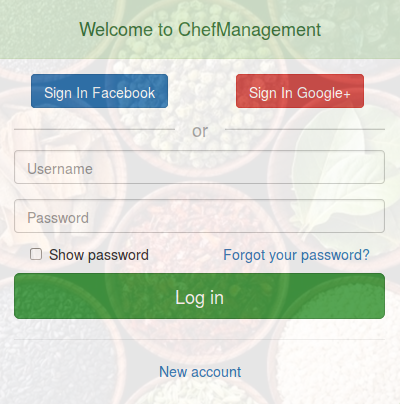
\includegraphics[width=8cm]{./images/chefmanagement-root.png}
	\caption{Acceso a la aplicación} \label{fig:chefmanagement-root}
\end{figure}

Además existe la opción de validarnos en la aplicación, una vez que se haya completado el registro. Si el usuario de entrada o contraseña fueran incorrectos la aplicación lo notificaría. En caso de pérdida de contraseña podemos solicitar una nueva accediendo al enlace \emph{Forgot your password?} y proporcionar nuestro nombre de usuario. Posteriormente puede modificarse la nueva contraseña en opciones~\ref{sec:cap.2.5}.

\begin{figure}[H]
	\centering
	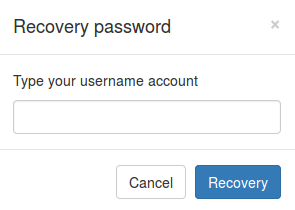
\includegraphics[width=8cm]{./images/chefmanagement-recovery.png}
	\caption{Registro} \label{fig:chefmanagement-recovery}
\end{figure}

Para registarse accedemos a través del enlace \emph{New account}. En caso de cualquier problema durante el proceso de registro, como que el correo o nombre de usuario estén en uso, la aplicación lo notificará al usuario.

\begin{figure}[H]
	\centering
	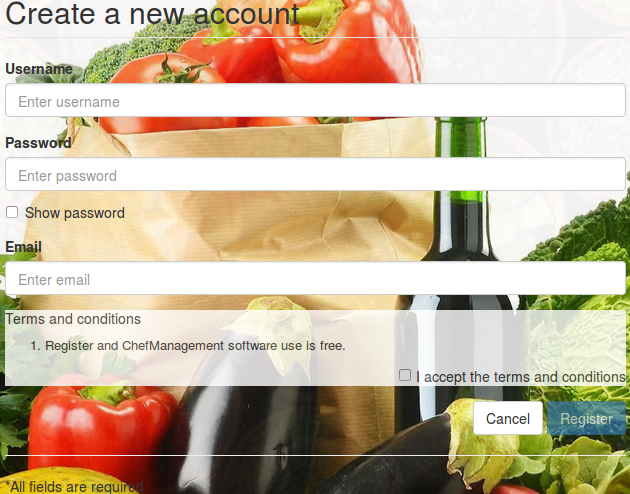
\includegraphics[width=8cm]{./images/chefmanagement-register.png}
	\caption{Registro} \label{fig:chefmanagement-register}
\end{figure}

Una vez dentro de la aplicación accederemos al \emph{home} del usuario. Existe un barra superior donde podemos acceder a la configuración y salir de la aplicación (Log out). También encontramos un menú lateral el cual facilita la interacción del usuario con la aplicación y ayudar a moverse y gestionar las distintas tareas. Por defecto, cuando accedemos a la aplicación, en \emph{home} se nos despliega la lista de recetas creadas por ese usuario. Las opciones del menú son las siguientes:

\begin{itemize}
	\item Recipe list: muestra el listado de recetas del usuario. Podemos acceder, editar y borrar recetas a través de esta lista.
	\item Recipe calculator: calcula el costo de producción de una receta y sus ingredientes para una determinada receta y raciones.
	\item New recipe: crea una nueva receta.
	\item Import: carga una copia de seguridad de las recetas del usuario.
	\item Export: almacena en el equipo local una copa de seguridad de las recetas del usuario.
\end{itemize}


\vspace*{0.2in}
\section{Crear recetas}\label{cap.2.2}

\vspace*{0.1in}
Para acceder a crear receta, nos situamos en el menú lateral y pinchamos en \textbf{New recipe}. Esto nos llevará a una nueva ventana, la cual presentará un formulario con una serie de campos que se detallan a continuación:

\begin{itemize}
	\item Name: es un campo obligatorio y clave primaria en la bbdd. Nombre de la receta.
	\item Rations: Numero de raciones para crear esa receta. Este campo es muy importante ya que se tomará como referencia para el cálculo de recetas dado un determinado número de platos.
	\item Cost: es un campo de lectura, se calcula acutomáticamente con cada ingrediente.
	\item Ration cost: relación entre el coste de la receta y el número de raciones.
	\item Order: campo que sirve como etiqueta. Indica si se trata de un primer o segundo plato, un postre, etc.
	\item Type: segundo campo de etiqueta. Nos da información sobre el tipo de comida: snack, comida casera y otros.
	\item Nivel: nivel de dificultad de producción de la receta.
	\item Time: horas y minutos que se estima que lleva preparar esa receta.
	\item Vegan: indica si la receta es apta para vegetarianos.
	\item Allergens: campo de texto para introducir alimentos que puedan producir alergias.
	\item Origin: información sobre el país originario de la receta.
\end{itemize}

Una vez completado podemos guardar la receta con el botón \textbf{Save recipe} o cancelar el proceso y volver a \emph{home}. Si guardamos la receta el sistema notificará de su registro en la bbdd y abrirá nuevos campos: 

\begin{itemize}
	\item Un área de texto desplegable que se utiliza para escribir las instrucciones de la receta. He utilizado la herramienta \href{http://ckeditor.com/}{ckeditor} para integrarla en la aplicación-
	\item Ingredientes, que puede ser:
		\begin{itemize}
			\item Un \textbf{nuevo ingrediente} creador por el usuario. Campos:
				\begin{itemize}
					\item Nombre del ingrediente
					\item Cantidad: puede ser: peso, volumen o una determinada unidad.
					\item Precio en relación con su cantidad
					\item El \% de merma o pérdida del ingrediente durante su preparación.
				\end{itemize}
			\item \textbf{Una receta} ya creada por el usuario. De forma que las recetas puedan servir de base para crear otras, por ejemplo, la salsa de tomate es una receta que se puede usar en otras. Si una receta usa otra, la primera no puede ser usada para crear otra y no aparecerá como opción en este apartado.
		\end{itemize}
\end{itemize}

A medida que vayamos incluyendo ingredientes a la receta, en el margen lateral derecho se desplegará una lista informativa de la receta con los ingredientes agregados hasta el momento.

\vspace*{0.2in}
\section{Editar y eliminar recetas}\label{cap.2.3}

\vspace*{0.1in}

\vspace*{0.2in}
\section{Calculadora}\label{cap.2.4}

\vspace*{0.1in}

\vspace*{0.2in}
\section{Importar y exportar}\label{cap.2.5}

\vspace*{0.1in}

\vspace*{0.2in}
\section{Opciones}\label{cap.2.5}

\vspace*{0.1in}

\vspace*{0.2in}
\section{Diseño de la base de datos}\label{cap.2.6}

\vspace*{0.1in}

\end{document}
